% Graphic for TeX using PGF
% Title: /home/lauri/msc-thesis/dia/traditional-partitioning.dia
% Creator: Dia v0.97.3
% CreationDate: Sun Apr  5 10:02:27 2015
% For: lauri
% \usepackage{tikz}
% The following commands are not supported in PSTricks at present
% We define them conditionally, so when they are implemented,
% this pgf file will use them.
\ifx\du\undefined
  \newlength{\du}
\fi
\setlength{\du}{15\unitlength}
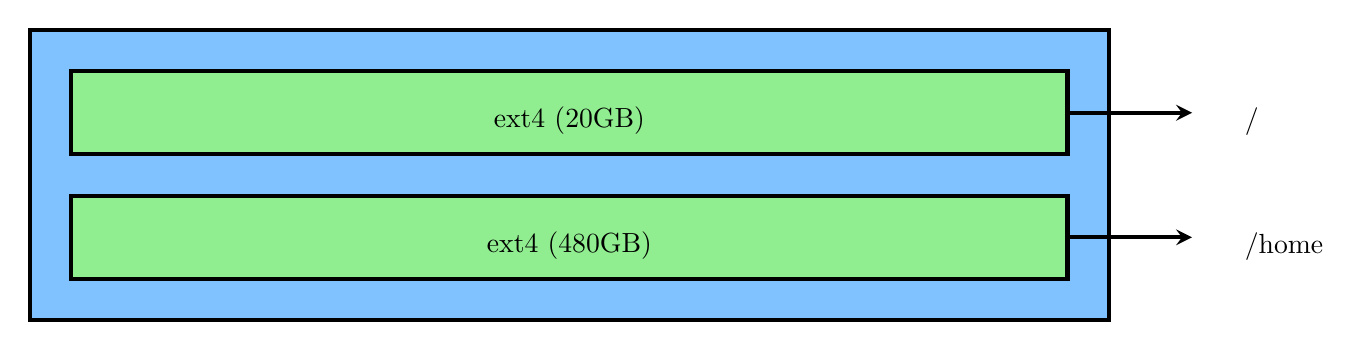
\begin{tikzpicture}
\pgftransformxscale{1.000000}
\pgftransformyscale{-1.000000}
\definecolor{dialinecolor}{rgb}{0.000000, 0.000000, 0.000000}
\pgfsetstrokecolor{dialinecolor}
\definecolor{dialinecolor}{rgb}{1.000000, 1.000000, 1.000000}
\pgfsetfillcolor{dialinecolor}
\pgfsetlinewidth{0.100000\du}
\pgfsetdash{}{0pt}
\pgfsetdash{}{0pt}
\pgfsetmiterjoin
\definecolor{dialinecolor}{rgb}{0.501961, 0.756863, 1.000000}
\pgfsetfillcolor{dialinecolor}
\fill (0.000000\du,0.000000\du)--(0.000000\du,7.000000\du)--(26.000000\du,7.000000\du)--(26.000000\du,0.000000\du)--cycle;
\definecolor{dialinecolor}{rgb}{0.000000, 0.000000, 0.000000}
\pgfsetstrokecolor{dialinecolor}
\draw (0.000000\du,0.000000\du)--(0.000000\du,7.000000\du)--(26.000000\du,7.000000\du)--(26.000000\du,0.000000\du)--cycle;
\definecolor{dialinecolor}{rgb}{0.564706, 0.933333, 0.564706}
\pgfsetfillcolor{dialinecolor}
\fill (1.000000\du,1.000000\du)--(1.000000\du,3.000000\du)--(25.000000\du,3.000000\du)--(25.000000\du,1.000000\du)--cycle;
\pgfsetlinewidth{0.100000\du}
\pgfsetdash{}{0pt}
\pgfsetdash{}{0pt}
\pgfsetmiterjoin
\definecolor{dialinecolor}{rgb}{0.000000, 0.000000, 0.000000}
\pgfsetstrokecolor{dialinecolor}
\draw (1.000000\du,1.000000\du)--(1.000000\du,3.000000\du)--(25.000000\du,3.000000\du)--(25.000000\du,1.000000\du)--cycle;
% setfont left to latex
\definecolor{dialinecolor}{rgb}{0.000000, 0.000000, 0.000000}
\pgfsetstrokecolor{dialinecolor}
\node at (13.000000\du,2.195000\du){ext4 (20GB)};
\pgfsetlinewidth{0.100000\du}
\pgfsetdash{}{0pt}
\pgfsetdash{}{0pt}
\pgfsetbuttcap
{
\definecolor{dialinecolor}{rgb}{0.000000, 0.000000, 0.000000}
\pgfsetfillcolor{dialinecolor}
% was here!!!
\pgfsetarrowsend{stealth}
\definecolor{dialinecolor}{rgb}{0.000000, 0.000000, 0.000000}
\pgfsetstrokecolor{dialinecolor}
\draw (25.000000\du,2.000000\du)--(28.000000\du,2.000000\du);
}
\pgfsetlinewidth{0.100000\du}
\pgfsetdash{}{0pt}
\pgfsetdash{}{0pt}
\pgfsetbuttcap
{
\definecolor{dialinecolor}{rgb}{0.000000, 0.000000, 0.000000}
\pgfsetfillcolor{dialinecolor}
% was here!!!
\pgfsetarrowsend{stealth}
\definecolor{dialinecolor}{rgb}{0.000000, 0.000000, 0.000000}
\pgfsetstrokecolor{dialinecolor}
\draw (25.000000\du,5.000000\du)--(28.000000\du,5.000000\du);
}
% setfont left to latex
\definecolor{dialinecolor}{rgb}{0.000000, 0.000000, 0.000000}
\pgfsetstrokecolor{dialinecolor}
\node[anchor=west] at (29.000000\du,5.221250\du){/home};
% setfont left to latex
\definecolor{dialinecolor}{rgb}{0.000000, 0.000000, 0.000000}
\pgfsetstrokecolor{dialinecolor}
\node[anchor=west] at (29.000000\du,2.221250\du){/};
\definecolor{dialinecolor}{rgb}{0.564706, 0.933333, 0.564706}
\pgfsetfillcolor{dialinecolor}
\fill (1.000000\du,4.000000\du)--(1.000000\du,6.000000\du)--(25.000000\du,6.000000\du)--(25.000000\du,4.000000\du)--cycle;
\pgfsetlinewidth{0.100000\du}
\pgfsetdash{}{0pt}
\pgfsetdash{}{0pt}
\pgfsetmiterjoin
\definecolor{dialinecolor}{rgb}{0.000000, 0.000000, 0.000000}
\pgfsetstrokecolor{dialinecolor}
\draw (1.000000\du,4.000000\du)--(1.000000\du,6.000000\du)--(25.000000\du,6.000000\du)--(25.000000\du,4.000000\du)--cycle;
% setfont left to latex
\definecolor{dialinecolor}{rgb}{0.000000, 0.000000, 0.000000}
\pgfsetstrokecolor{dialinecolor}
\node at (13.000000\du,5.195000\du){ext4 (480GB)};
\end{tikzpicture}
